%% BioMed_Central_Tex_Template_v1.06
%%                                      %
%  bmc_article.tex            ver: 1.06 %
%                                       %

%%IMPORTANT: do not delete the first line of this template
%%It must be present to enable the BMC Submission system to
%%recognise this template!!

%%%%%%%%%%%%%%%%%%%%%%%%%%%%%%%%%%%%%%%%%
%%                                     %%
%%  LaTeX template for BioMed Central  %%
%%     journal article submissions     %%
%%                                     %%
%%          <8 June 2012>              %%
%%                                     %%
%%                                     %%
%%%%%%%%%%%%%%%%%%%%%%%%%%%%%%%%%%%%%%%%%


%%%%%%%%%%%%%%%%%%%%%%%%%%%%%%%%%%%%%%%%%%%%%%%%%%%%%%%%%%%%%%%%%%%%%
%%                                                                 %%
%% For instructions on how to fill out this Tex template           %%
%% document please refer to Readme.html and the instructions for   %%
%% authors page on the biomed central website                      %%
%% http://www.biomedcentral.com/info/authors/                      %%
%%                                                                 %%
%% Please do not use \input{...} to include other tex files.       %%
%% Submit your LaTeX manuscript as one .tex document.              %%
%%                                                                 %%
%% All additional figures and files should be attached             %%
%% separately and not embedded in the \TeX\ document itself.       %%
%%                                                                 %%
%% BioMed Central currently use the MikTex distribution of         %%
%% TeX for Windows) of TeX and LaTeX.  This is available from      %%
%% http://www.miktex.org                                           %%
%%                                                                 %%
%%%%%%%%%%%%%%%%%%%%%%%%%%%%%%%%%%%%%%%%%%%%%%%%%%%%%%%%%%%%%%%%%%%%%

%%% additional documentclass options:
%  [doublespacing]
%  [linenumbers]   - put the line numbers on margins

%%% loading packages, author definitions

\documentclass[twocolumn]{bmcart}% uncomment this for twocolumn layout and comment line below
%\documentclass{bmcart}

%%% Load packages
\usepackage{amsthm,amsmath}
\usepackage{siunitx}
\usepackage{mfirstuc}
%\RequirePackage{natbib}
\usepackage[colorinlistoftodos]{todonotes}
\RequirePackage{hyperref}
\usepackage[utf8]{inputenc} %unicode support
%\usepackage[applemac]{inputenc} %applemac support if unicode package fails
%\usepackage[latin1]{inputenc} %UNIX support if unicode package fails
\usepackage[htt]{hyphenat}

\usepackage{array}
\newcolumntype{L}[1]{>{\raggedright\let\newline\\\arraybackslash\hspace{0pt}}p{#1}}

%%%%%%%%%%%%%%%%%%%%%%%%%%%%%%%%%%%%%%%%%%%%%%%%%
%%                                             %%
%%  If you wish to display your graphics for   %%
%%  your own use using includegraphic or       %%
%%  includegraphics, then comment out the      %%
%%  following two lines of code.               %%
%%  NB: These line *must* be included when     %%
%%  submitting to BMC.                         %%
%%  All figure files must be submitted as      %%
%%  separate graphics through the BMC          %%
%%  submission process, not included in the    %%
%%  submitted article.                         %%
%%                                             %%
%%%%%%%%%%%%%%%%%%%%%%%%%%%%%%%%%%%%%%%%%%%%%%%%%


%\def\includegraphic{}
%\def\includegraphics{}

%%% Put your definitions there:
\startlocaldefs
\endlocaldefs


%%% Begin ...
\begin{document}

%%% Start of article front matter
\begin{frontmatter}

\begin{fmbox}
\dochead{Report from Brainhack}

%%%%%%%%%%%%%%%%%%%%%%%%%%%%%%%%%%%%%%%%%%%%%%
%%                                          %%
%% Enter the title of your article here     %%
%%                                          %%
%%%%%%%%%%%%%%%%%%%%%%%%%%%%%%%%%%%%%%%%%%%%%%

\title{Missing Title}
\vskip2ex
URL is missing}


%%%%%%%%%%%%%%%%%%%%%%%%%%%%%%%%%%%%%%%%%%%%%%
%%                                          %%
%% Enter the authors' addresses here        %%
%%                                          %%
%% Repeat \address commands as much as      %%
%% required.                                %%
%%                                          %%
%%%%%%%%%%%%%%%%%%%%%%%%%%%%%%%%%%%%%%%%%%%%%%


%%%%%%%%%%%%%%%%%%%%%%%%%%%%%%%%%%%%%%%%%%%%%%
%%                                          %%
%% Enter short notes here                   %%
%%                                          %%
%% Short notes will be after addresses      %%
%% on first page.                           %%
%%                                          %%
%%%%%%%%%%%%%%%%%%%%%%%%%%%%%%%%%%%%%%%%%%%%%%

\begin{artnotes}
\end{artnotes}

%\end{fmbox}% comment this for two column layout

%%%%%%%%%%%%%%%%%%%%%%%%%%%%%%%%%%%%%%%%%%%%%%
%%                                          %%
%% The Abstract begins here                 %%
%%                                          %%
%% Please refer to the Instructions for     %%
%% authors on http://www.biomedcentral.com  %%
%% and include the section headings         %%
%% accordingly for your article type.       %%
%%                                          %%
%%%%%%%%%%%%%%%%%%%%%%%%%%%%%%%%%%%%%%%%%%%%%%

%\begin{abstractbox}

%\begin{abstract} % abstract
	
%Blank Abstract

%\end{abstract}



%%%%%%%%%%%%%%%%%%%%%%%%%%%%%%%%%%%%%%%%%%%%%%
%%                                          %%
%% The keywords begin here                  %%
%%                                          %%
%% Put each keyword in separate \kwd{}.     %%
%%                                          %%
%%%%%%%%%%%%%%%%%%%%%%%%%%%%%%%%%%%%%%%%%%%%%%

%\vskip1ex

%URL is missing}
%URL is missing}

% MSC classifications codes, if any
%\begin{keyword}[class=AMS]
%\kwd[Primary ]{}
%\kwd{}
%\kwd[; secondary ]{}
%\end{keyword}

%\end{abstractbox}
%
\end{fmbox}% uncomment this for twcolumn layout

\end{frontmatter}

%{\sffamily\bfseries\fontsize{10}{12}\selectfont Project URL: \url{}}

%%% Import the body from pandoc formatted text
\section{Introduction}\label{introduction}

Resting-state fMRI (rsfMRI) data generates interesting time courses with
unpredictable hills and valleys. This data in some degree resembles the
notes of a music scale. Taking advantage of these similarities and using
only the rsfMRI data as input, we use basic rules of music theory to
transform the data into pleasant music. Our project is implemented in
Python using the \href{https://code.google.com/p/midiutil/}{midiutil
library}.

\section{Approach}\label{approach}

\textit{Data}: We used open rsfMRI from the ABIDE dataset
\cite{di2014autism} preprocessed by the Preprocessed Connectomes Project
\cite{pcp}. We randomly chose 10 subjects preprocessed using C-PAC
pipeline \cite{Craddock2013c} with 4 different strategies. For reducing
the data dimensionality, we chose the CC200 atlas \cite{cc200}.

\textit{Processing:} fMRI time courses were analysed to extract pitch,
tempo, and volume - 3 important attributes for generating music. For
pitch, we mapped the time course amplitudes to MIDI values in the range
of 36 to 84, corresponding to piano keys in within a pentatonic scale.
The key of the scale is determined by the global mean ROI value
(calculated across all timepoints and ROIs) using the equation:
\texttt{(global signal \% 49) + 36}. The lowest tone that can be played
in a certain key is calculated from \texttt{(key \% 12) + 36}. The set
of tones that can be played are then determined from the lowest tone
using a scale. For example, the minor-pentatonic scale's set of tones is
calculated by adding \texttt{[0, 3, 5, 7, 10]} to its lowest tone, then
skipping to the next octave, and then repeating the process until the
value 84 is reached. An fMRI time course is mapped to these possible
tones by scaling its amplitude to the range between the smallest and
largest tones in the set. If a time point maps to a tone that is not in
the set, it is shifted to the closest allowable tone. An example of
allowed set of tones is shown in Figure \ref{keyfig}.

For tempo, we use the first temporal derivative for calculating the
length of notes, assuming we have 4 lengths (whole, half, quarter and
eighth note). In the time course, if the modulus distance between time
point \textit{t} and \textit{t + 1} is big, we interpret it as a fast
note (eighth). However, if the distance between \textit{t} and
\textit{t + 1} is close to zero, we assume it is a slow note (whole).
Using this approach, we map all the other notes in between.

We use a naive approach for calculating volume in a way that tackles a
problem we have with fast notes: their sound is cut off due to their
short duration. An simple way to solve this is to decrease the volume of
fast notes. Thus, the faster the note, the lower the volume. While a
whole note has volume 100 ({[}0,100{]}), an eighth note has volume 50.

Finally, we choose the brain regions that will play. Users complain when
two similar brain regions play together. Apparently, the brain produces
the same music twice. However, when the regions are distinct, the music
is pleasant. Thus, we use FastICA \cite{scikitlearn} for choosing brain
regions with maximally uncorrelated time courses.

\section{Results}\label{results}

A framework for generating music from fMRI data, based on music theory,
was developed and implemented as a Python tool yielding several audio
files. When listening to the results, we noticed that music across
subjects is different. However, music generated by the same subject (4
preprocessing strategies) sounds similar. Our results sound different
from music obtained in a similar study using EEG and fMRI data
\cite{lu2012scale}.

\section{Conclusions}\label{conclusions}

In this experiment, we established a way of generating music with open
fMRI data following some basic music theory principles. This resulted in
a somewhat naïve but pleasant music for humans. The results show an
interesting possibility for providing feedback of fMRI activity for
neurofeedback experiments.

\begin{figure}
  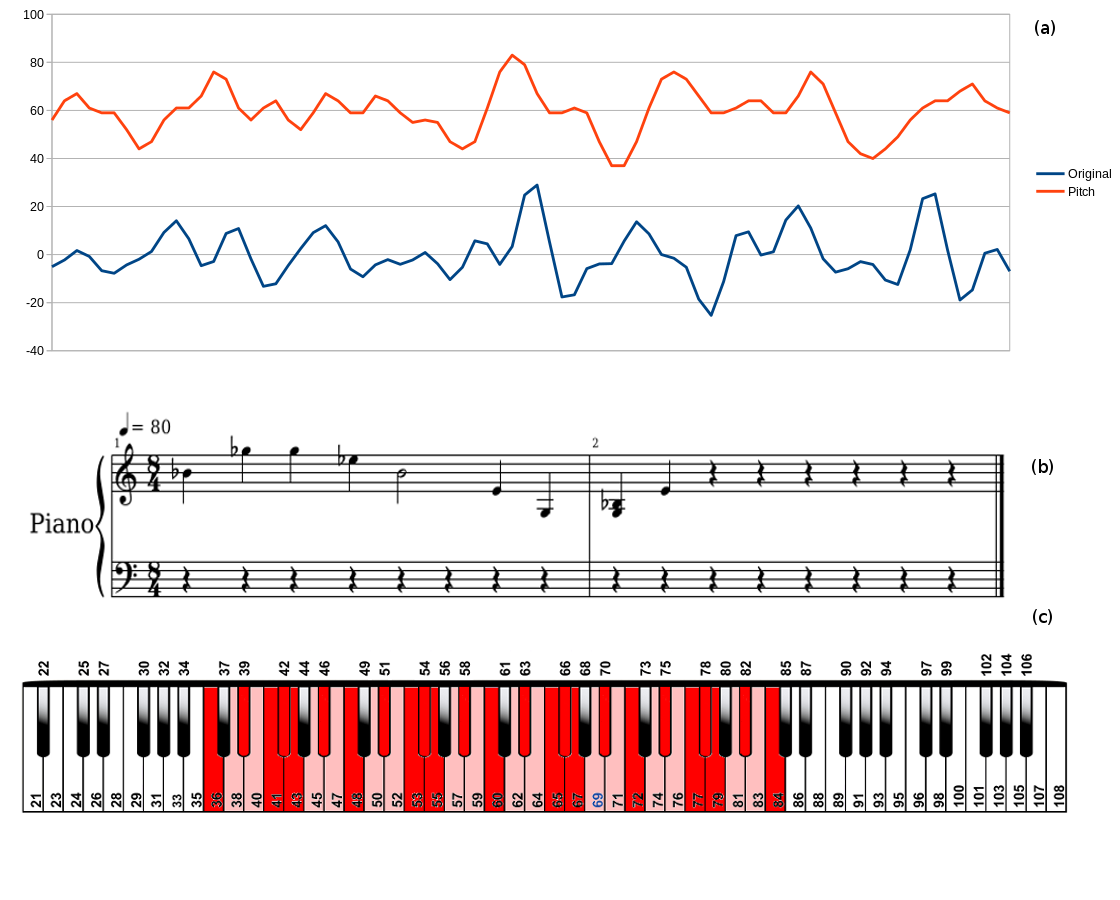
\includegraphics[width=0.45\textwidth]{figure}
  \caption{\label{keyfig}
  (a)Correspondence between the original time series of one ROI and the generated pitch.
  (b)The first 10 notes of the same ROI as sheet music.
  (c)All possible piano keys the brain can play, from 36 to 84 (in pink).
    We show in red all the possible tones for a C Minor-pentatonic scale, in the range of [36, 84].
    In that case, the lowest key is 36.
    The keys that can be used are: [36, 39, 41, 42, 43, 46, 48, 51, 53, 54, 55, 58, 60, 63, 65, 66, 67, 70, 72, 75, 77, 78, 79, 82, 84]
      }
\end{figure}

%%%%%%%%%%%%%%%%%%%%%%%%%%%%%%%%%%%%%%%%%%%%%%
%%                                          %%
%% Backmatter begins here                   %%
%%                                          %%
%%%%%%%%%%%%%%%%%%%%%%%%%%%%%%%%%%%%%%%%%%%%%%

\begin{backmatter}

\section*{Availability of Supporting Data}
More information about this project can be found at: \emph{URL is missing} 

\section*{Competing interests}
\emph{Competing interests statement is missing.}

\section*{Author's contributions}
\emph{Author's contributions statement is missing.}

\section*{Acknowledgements}
\emph{Acknowedgements section is missing.}

  
  
%%%%%%%%%%%%%%%%%%%%%%%%%%%%%%%%%%%%%%%%%%%%%%%%%%%%%%%%%%%%%
%%                  The Bibliography                       %%
%%                                                         %%
%%  Bmc_mathpys.bst  will be used to                       %%
%%  create a .BBL file for submission.                     %%
%%  After submission of the .TEX file,                     %%
%%  you will be prompted to submit your .BBL file.         %%
%%                                                         %%
%%                                                         %%
%%  Note that the displayed Bibliography will not          %%
%%  necessarily be rendered by Latex exactly as specified  %%
%%  in the online Instructions for Authors.                %%
%%                                                         %%
%%%%%%%%%%%%%%%%%%%%%%%%%%%%%%%%%%%%%%%%%%%%%%%%%%%%%%%%%%%%%

% if your bibliography is in bibtex format, use those commands:

\end{backmatter}
\end{document}
